\let\lesson\undefined
\newcommand{\lesson}{\phantomlesson{Bài 7: Gia tốc. Chuyển động thẳng biến đổi đều}}
\chapter[Chuyển động thẳng biến đổi đều]{Chuyển động thẳng biến đổi đều}
\setcounter{section}{0}
\section{Lý thuyết}
\subsection{Chuyển động thẳng biến đổi đều}

Chuyển động thẳng biến đổi đều là chuyển động có 
\begin{itemize}
	\item quỹ đạo là đường thẳng
	\item độ lớn của vận tốc tức thời tăng đều hoặc giảm đều theo thời gian.
\end{itemize}  
\begin{center}
	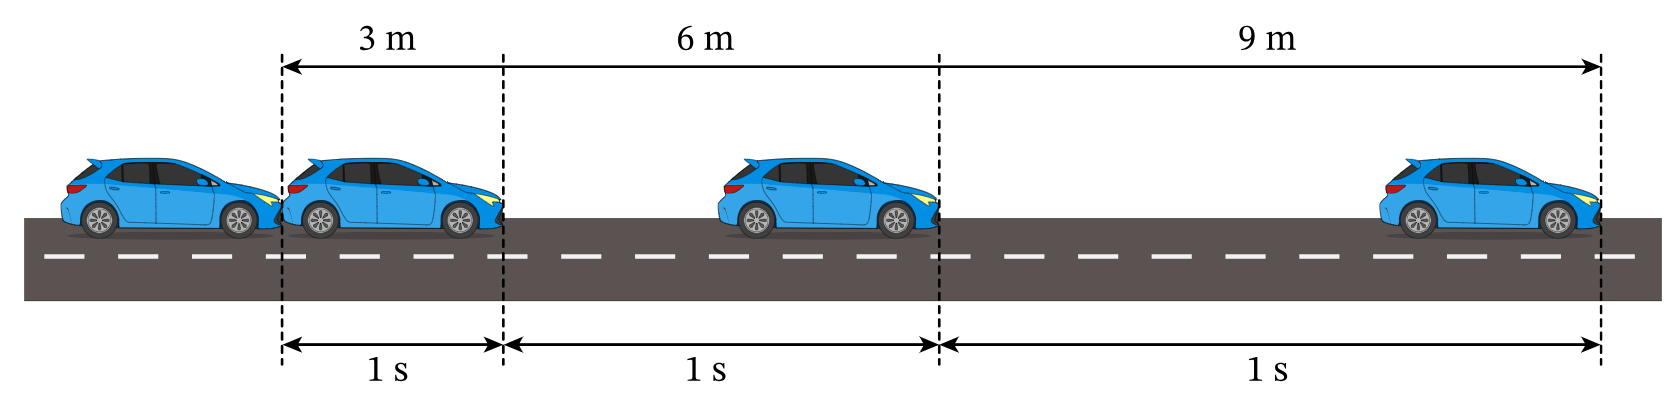
\includegraphics[width=0.75\linewidth]{../figs/VN10-2023-PH-TP009-1}
	\captionof{figure}{Minh hoạ chuyển động thẳng biến đổi đều của một ô tô với gia tốc $\SI{3}{\meter/\second^2}$.}
\end{center}
\begin{center}
	\begin{tabular}{|m{20em}|m{20em}|}
		\hline
		\thead{Chuyển động thẳng nhanh dần đều} & \thead{Chuyển động thẳng chậm dần đều}\\
		\hline
		Tốc độ tăng đều theo thời gian & Tốc độ giảm đều theo thời gian\\
		$\vec{a}$ và $\vec{v}$ cùng chiều, $a\cdot v>0$ & $\vec{a}$ và $\vec{v}$ ngược chiều, $a\cdot v<0$\\
		\hline
	\end{tabular}
\end{center}
\subsection{Các phương trình của chuyển động thẳng biến đổi đều}
\subsubsection{Phương trình gia tốc}
$$a=\text{hằng số}$$
\luuy{Nếu chọn chiều chuyển động là chiều dương
\begin{itemize}
	\item $a>0$: vật chuyển động nhanh dần đều.
	\item $a<0$: vật chuyển động chậm dần đều.
\end{itemize}}
\subsubsection{Phương trình vận tốc}
Xét tại thời điểm $t_0=0$, vật chuyển động với vận tốc $v_0$ và gia tốc $a$. Tại thời điểm $t$, vật có vận tốc 
	\begin{equation}
		v=v_0+at,
	\end{equation}
Trong chuyển động thẳng biến đổi đều gia tốc $a$ có giá trị không đổi, vận tốc tức thời $v$ là hàm bậc nhất theo $t$ nên đồ thị vận tốc - thời gian có dạng là một nửa đường thẳng.
\begin{center}
	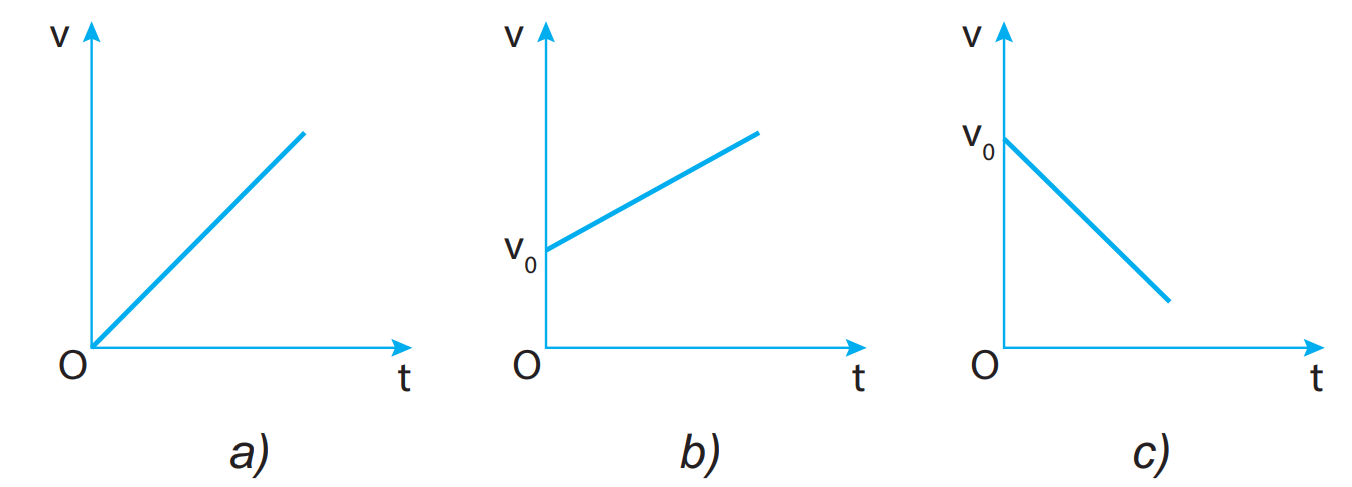
\includegraphics[width=0.6\linewidth]{../figs/VN10-2023-PH-TP009-2}
	\captionof{figure}{Đồ thị vận tốc - thời gian của vật chuyển động thẳng biến đổi đều.
	\textit{Hình a)} Vật chuyển động nhanh dần đều từ trạng thái nghỉ; \textit{Hình b)} Vật chuyển động thẳng nhanh dần đều, \textit{Hình c)} Vật chuyển động thẳng chậm dần đều.}
\end{center}
Nếu trong quá trình chuyển động vật có đổi chiều chuyển động thì đồ thị vận tốc - thời gian có dạng:\\
\begin{minipage}[l]{10cm}
	\begin{center}
		\begin{tikzpicture}
			\coordinate (O) at (0,0);
			\coordinate (xaxis) at (5,0);
			\coordinate (ydaxis) at (0,-2);
			\coordinate (yuaxis) at (0,2);
			\draw[->,name path=Ox] (O)--(xaxis);
			\draw[->,name path=Oy] (ydaxis)--(yuaxis);
			\node[below left] at (O) {O};
			\node[above left] at (yuaxis) {$v$ };
			\node[right] at (xaxis) {$t$ };
			\path (0,-1.5) coordinate (vo) node[left] {$v_0$};
			\path (4,1.5) coordinate (v) node[left] {};
			\draw[thick,blue,name path=line] (vo)--(v);
			\node[above,text width=2.5cm,align=center] (1) at (2,1.5) {\small{nhanh dần đều }\\$a\cdot v>0$};
			\draw[->] (1.south) to [bend right] (2.7,0.8);
			\node[below,text width=1.5cm,align=center] (2) at (3.5,0) {\small{dừng lại}\\$v=0$};
			\path [name intersections={of=Ox and line,by=E}];
			\filldraw[red] (E) circle (2pt);
			\draw[->] (2.west) to [bend left] (2.05,-0.1);
			\node[below,text width=2.5cm,align=center] (3) at (3.5,-1.5) {\small{chậm dần đều}\\$a\cdot v<0$};
			\draw[->] (3.west) to [bend left] (1,-1);
		\end{tikzpicture}
	\captionof{figure}{Đồ thị hướng lên trên: $a>0$}
	\end{center}
\end{minipage}
\begin{minipage}[l]{10cm}
	\begin{center}
		\begin{tikzpicture}
			\coordinate (O) at (0,0);
			\coordinate (xaxis) at (5,0);
			\coordinate (ydaxis) at (0,-2);
			\coordinate (yuaxis) at (0,2);
			\draw[->,name path=Ox] (O)--(xaxis);
			\draw[->,name path=Oy] (ydaxis)--(yuaxis);
			\node[below left] at (O) {O};
			\node[above left] at (yuaxis) {$v$ };
			\node[right] at (xaxis) {$t$ };
			\path (0,1.5) coordinate (vo) node[left] {$v_0$};
			\path (4,-1.5) coordinate (v) node[left] {};
			\draw[thick,blue,name path=line] (vo)--(v);
			\node[above,text width=2.5cm,align=center] (1) at (2.5,1.5) {\small{chậm dần đều }\\$a\cdot v<0$};
			\draw[->] (1.south) to [bend left] (1.2,0.8);
			\node[below,text width=1.2cm,align=center] (2) at (0.8,0) {\small{dừng lại}\\$v=0$};
			\path [name intersections={of=Ox and line,by=E}];
			\filldraw[red] (E) circle (2pt);
			\draw[->] (2.east) to [bend right] (2,-0.1);
			\node[below,text width=2.5cm,align=center] (3) at (1.2,-1.5) {\small{nhanh dần đều}\\$a\cdot v>0$};
			\draw[->] (3.east) to [bend right] (3,-1);
		\end{tikzpicture}
	\captionof{figure}{Đồ thị hướng xuống dưới: $a<0$}
		\end{center}
\end{minipage}
\subsection{Phương trình độ dịch chuyển}
\begin{center}
	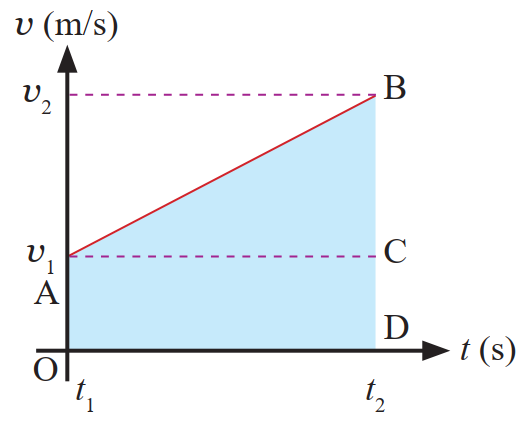
\includegraphics[width=0.3\linewidth]{../figs/VN10-2023-PH-TP008-4}
	\captionof{figure}{Đồ thị $\left(v - t\right)$ của vật chuyển động thẳng biến đổi đều.}
	\label{fig:9.3}
\end{center}
Dựa vào đồ thị $\left(v - t\right)$ Hình \ref{fig:9.3} của vật chuyển động thẳng biến đổi đều. Ta có độ dịch chuyển trong khoảng thời gian $\Delta t= t- 0 =t$ chính là diện tích hình thang $OABD$:
$$d=\dfrac{1}{2}\left(OA+BD\right)\cdot OD=\dfrac{1}{2}\left(v+v_0\right)\cdot t$$
Mà $v=v_0+at$
Ta rút ra được phương trình độ dịch chuyển của vật:
$$d=v_0\cdot t+\dfrac{1}{2}a\cdot t^2$$
Đồ thị $\left(d - t\right)$ của chuyển động thẳng biến đổi đều được biểu diễn trong Hình \ref{fig:9.4} là một nhánh parabol.
\begin{center}
	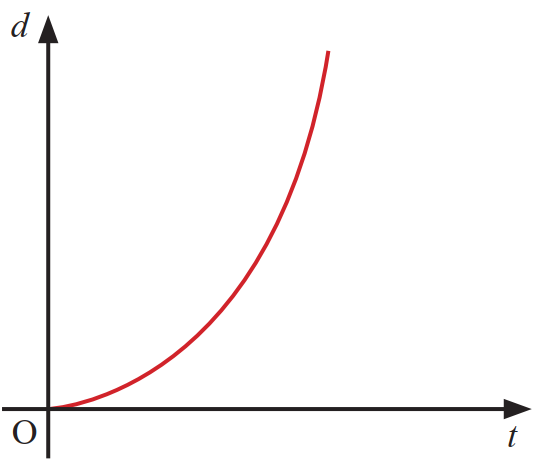
\includegraphics[width=0.3\linewidth]{../figs/VN10-2023-PH-TP009-4}
	\captionof{figure}{Đồ thị $\left(d - t\right)$ của vật chuyển động thẳng biến đổi đều.}
	\label{fig:9.4}
\end{center}
Nếu tại thời điểm $t_0$, vật ở vị trí $x_0$ so với gốc toạ độ. Do $d=x-x_0$, ta rút ra được phương trình xác định toạ độ của vật chuyển động thẳng biến đổi đều
$$x=x_0+v_0\cdot t+\dfrac{1}{2}a\cdot t^2$$
trong đó:
\begin{itemize}[label=$\circ$]
	\item $x_0$: tọa độ ban đầu của vật tại thời điểm $t_0$;
	\item $x$: tọa độ của vật tại thời điểm $t$;
	\item $v_0$: vận tốc của vật ($v_0>0$ nếu vật chuyển động cùng chiều dương, $v_0<0$ nếu vật chuyển động ngược chiều dương);
	\item $a$: gia tốc của vật ($a\cdot v_0>0$ nếu vật chuyển động nhanh dần đều, $a\cdot v_0<0$ nếu vật chuyển động chậm dần đều).
\end{itemize}
\subsection{Phương trình liên hệ giữa gia tốc, vận tốc và độ dịch chuyển}
$$v^2-v^2_0=2a\cdot d$$

\section{Mục tiêu bài học - Ví dụ minh họa}
\begin{dang}{Nhận biết được đặc điểm \\của chuyển động thẳng biến đổi đều}
	\viduii{1}{Chuyển động thẳng biến đổi đều là chuyển động
		\begin{mcq}
			\item có quỹ đạo là đường thẳng, vectơ gia tốc bằng không.
			\item có quỹ đạo là đường thẳng, vectơ gia tốc không thay đổi trong suốt quá trình chuyển động.
			\item có quỹ đạo là đường thẳng, vectơ gia tốc và vận tốc không thay đổi trong suốt quá trình chuyển động.
			\item có quỹ đạo là đường thẳng, vectơ vận tốc không thay đổi trong suốt quá trình chuyển động.
		\end{mcq}
	}
	{\hide{
		Chuyển động thẳng biến đổi đều là chuyển động có quỹ đạo là đường thẳng, vectơ gia tốc không thay đổi trong suốt quá trình chuyển động.
		
		\textbf{Đáp án: B}.
	}}

\viduii{1}{Đồ thị nào sau đây là của chuyển động thẳng biến đổi?
	\begin{center}
		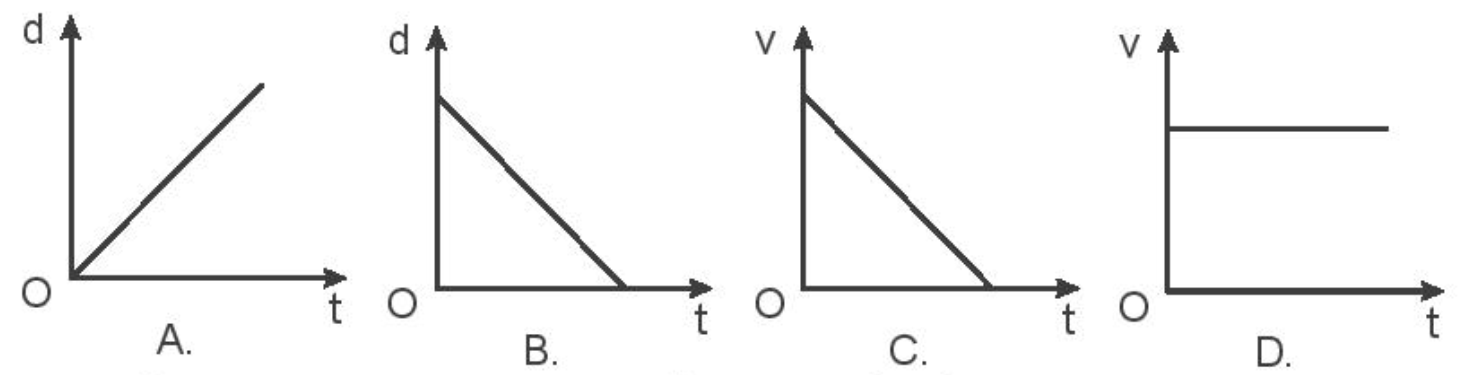
\includegraphics[width=0.6\linewidth]{../figs/VN10-2023-PH-TP009-5}
	\end{center}
}
{\hide{
Hình a) và b): Đồ thị $\left(d - t\right)$ là một đường thẳng thay đổi theo $t$, do đó đây là chuyển động thẳng đều.\\
Hình d): Đồ thị $\left( v - t\right)$ là một đường thẳng song song với trục $Ot$. Do đó, vận tốc không thay đổi theo thời gian. Đây là chuyển động thẳng đều.\\
Hình c): Đồ thị $\left(v - t\right)$ là có dạng đường thẳng thay đổi theo $t$. Do đó, vận tốc là hàm bậc nhất của thời gian. Đây là chuyển động thẳng biến đổi đều.
}}
\end{dang}


\begin{dang}{Áp dụng được công thức liên hệ \\giữa độ dời, vận tốc, gia tốc }
	\viduii{2}{Một xe máy đang đi với $v = \SI{50,4}{km/h}$ bỗng người lái xe thấy có ổ gà trước mắt cách xe $\SI{24,5}{m}$. Người ấy phanh gấp và xe đến ổ gà thì dừng lại.
		\begin{enumerate}[label=\alph*.]
			\item Tính gia tốc.
			\item Tính thời gian phanh.
		\end{enumerate}
	}
	{\hide{
		Đơn vị vận tốc được đổi về hệ SI $$\SI{50,4}{\kilo\meter/\hour} =\dfrac{\SI{50.4e3}{\meter}}{\SI{3600}{\second}}= \SI{14}{m/s}.$$
		\begin{enumerate}[label=\alph*.]
			\item Gia tốc của xe máy
			$$v^2-v_0^2 =2a\cdot d \Rightarrow a =\dfrac{v^2 - v_0^2}{2d}=\dfrac{\left(\SI{0}{\meter/\second}\right)^{2}-\left(\SI{14}{\meter/\second}\right)^{2}}{2\cdot\SI{24.5}{\meter}}=\SI{-4}{m/s}^2.$$
			\item Thời gian phanh
			
			$$v =v_0 +at \Rightarrow t = \dfrac{v-v_0}{a} =\dfrac{\SI{0}{\meter/\second}-\SI{14}{\meter/\second}}{\SI{-4}{\meter/\second^{2}}}= \SI{3,5}{s}.$$
		\end{enumerate}
	}}

	\viduii{2}{Một đoàn tàu bắt đầu chuyển động nhanh dần đều khi đi hết $\SI{1}{km}$ đầu tiên thì đạt vận tốc $v=\SI{10}{m/s}$. Tính vận tốc đoàn tàu sau khi đi hết $\SI{2}{km}$.
	}
	{\hide{
		Gia tốc của đoàn tàu
		$$v^2-v_0^2 =2a\cdot d_1 \Rightarrow a = \dfrac{v^2-v_0^2}{2d_1}=\dfrac{\left(\SI{10}{\meter/\second}\right)^2-(\SI{0}{\meter/\second})^2}{2\cdot\SI{1000}{\meter}} =\SI{0,05}{m/s}^2.$$
		
		Vận tốc sau khi đi hết $\SI{2}{km}$
		$$v_1^2 - v_0^2 = 2a\cdot d_2 \Rightarrow  v_1 =\sqrt{2ad_2+v_0^2}=\sqrt{2\cdot\SI{0.05}{\meter/\second^{2}}\cdot\SI{2}{\kilo\meter}+\left(\SI{0}{\kilo\meter/\second^{2}}\right)^{2}} =\xsi{10\sqrt{2}}{\meter/\second}.$$
	}}
\end{dang}
\begin{dang}{Xây dựng đồ thị vận tốc - thời gian của vật chuyển động thẳng biến đổi đều}
	\viduii{3}{
		Một vật chuyển động có đồ thị vận tốc như hình vẽ. Công thức vận tốc và công thức đường đi của vật là
		\begin{center}
			\begin{tikzpicture}
				\coordinate (O) at (0,0);
				\coordinate (xaxis) at (3.5,0);
				\coordinate (yaxis) at (0,3);
				\draw[->] (O)--(xaxis);
				\draw[->] (O)--(yaxis);
				\node[below left] at (O) {O};
				\node[above] at (yaxis) {$v$ (m/s)};
				\node[right] at (xaxis) {$t$ (s)};
				\path (0,1) coordinate (vo) node[left] {20};
				\coordinate (v) at ($(vo)+(30:3)$);
				\coordinate (vt) at ($(vo)+(30:2)$);
				\draw[thick,blue] (vo)--(v);
				\path let \p1=(vt) in (\x1,0) coordinate (vtx) node[below] {20};
				\path let \p1=(vt) in (0,\y1) coordinate (vty) node[left] {40};
				\draw[dashed] (vt)--(vtx);
				\draw[dashed] (vt)--(vty); 
			\end{tikzpicture}
		\end{center}
		\begin{mcq}(2)
			\item $v=t$, $s=\dfrac{1}{2}t^2$.
			\item $v=20+t$, $s=20t+\dfrac{1}{2}t^2$.
			\item $v=20-t$, $s=20t-\dfrac{1}{2}t^2$.
			\item $v=40-2t$, $s=40t-\dfrac{1}{2}t^2$.
		\end{mcq}
	}
	{\hide{
		Đồ thị vận tốc - thời gian có dạng đường thẳng với hệ số góc khác không nên đây là đồ thị mô tả chuyển động thẳng biến đổi đều. 
		
		Gia tốc của vật được tính theo công thức
		\begin{equation*}
			a=\dfrac{v-v_0}{t}=\dfrac{\SI{40}{\meter/\second}-\SI{20}{\meter/\second}}{\SI{20}{\second}}=\SI{1}{\meter/\second^2}.
		\end{equation*}
		
		Phương trình vận tốc có dạng 
		\begin{equation*}
			v=v_0+at=20+t\textrm{ (m/s, s)}.
		\end{equation*}
		
		Công thức tính quãng đường đi được 
		\begin{equation*}
			s=v_0 t+\dfrac{1}{2}at^2=20t+\dfrac{1}{2}t^2\textrm{ (m, s)}.
		\end{equation*}
		
		\textbf{Đáp án: B}.
	}}

	\viduii{3}{Một xe đạp đang chuyển động với vận tốc $\SI{5}{\meter/\second}$ thì hãm phanh chuyển động chậm dần đều có đồ thị vận tốc theo thời gian sau. Tính quãng đường đi được từ lúc hãm phanh cho đến khi dừng lại.
		
		\begin{center}
			\begin{tikzpicture}
				\coordinate (O) at (0,0);
				\coordinate (xaxis) at (4,0);
				\coordinate (yaxis) at (0,3);
				\draw[->] (O)--(xaxis);
				\draw[->] (O)--(yaxis);
				\node[below left] at (O) {O};
				\node[above] at (yaxis) {$v$ (m/s)};
				\node[right] at (xaxis) {$t$ (s)};
				\path (0,2) coordinate (vo) node[left] {5};
				\path (3,0) coordinate (v) node[below] {10};
				\draw[thick,blue] (vo)--(v);
			\end{tikzpicture}
		\end{center}
	}
	{\hide{
		Gia tốc của vật là
		\begin{equation*}
			a=\dfrac{v-v_0}{t}=\dfrac{0-\SI{5}{\meter/\second}}{\SI{10}{\second}}=-\SI{0.5}{\meter/\second^2}.
		\end{equation*}
		
		Quãng đường đi được từ lúc hãm phanh cho đến khi dừng lại là:
		\begin{equation*}
			v^2-v_0^2=2a\cdot d\quad\Rightarrow\quad  s=\dfrac{v^2-v_0^2}{2a}=\dfrac{(\SI{0}{\meter/\second})^{2}-(\SI{5}{\meter/\second})^2}{2\cdot (\SI{-0.5}{\meter/\second^2})}=\SI{25}{\meter}.
		\end{equation*}
	}}

	\viduii{3}{Đồ thị vận tốc thời gian của một vật chuyển động như hình vẽ bên.
		\begin{center}
			\begin{tikzpicture}[scale=0.7]
				\coordinate (O) at (0,0);
				\coordinate (xaxis) at (7,0);
				\coordinate (yaxis) at (0,4);
				\draw[->] (O)--(xaxis);
				\draw[->] (O)--(yaxis);
				\node[below left] at (O) {O};
				\node[left] at (yaxis) {$v$ (m/s)};
				\node[right] at (xaxis) {$t$ (s)};
				\coordinate (A) at (0,2);
				\coordinate (B) at (1,3);
				\coordinate (C) at (3,3);
				\coordinate (D) at (6,0);				\node[right] at  (A) {A};
				\node[above] at (B) {B};
				\node[above] at (C) {C};
				\node[above right] at (D) {D};
				\draw[thick,blue] (A)--(B)--(C)--(D);
				\path let \p1=(B) in (\x1,0) coordinate (bd) node[below] {10};
				\path let \p2=(C) in (\x2,0) coordinate (cd) node[below] {30};
				\path let \p3=(B) in (0,\y3) coordinate (bl) node[left] {15};
				\node[left] at (A) {10};
				\node[below] at (D) {60};
				\draw[dashed] (B)--(bd);
				\draw[dashed] (C)--(cd);
				\draw[dashed] (B)--(bl);
			\end{tikzpicture}
			%			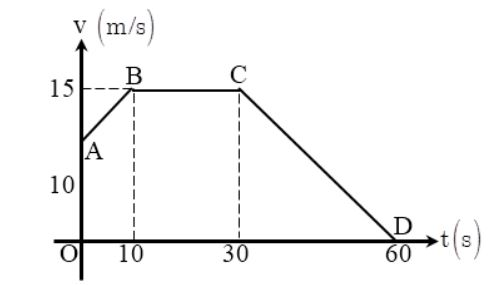
\includegraphics[scale=0.8]{../figs/VN10-PH-04-L-003-3-V2-04.jpg}
		\end{center}
		\begin{enumerate}[label=\alph*.]
			\item Nêu tính chất chuyển động của mỗi giai đoạn.
			\item Lập phương trình vận tốc của mỗi giai đoạn.
		\end{enumerate}
		
	}
	{\hide{
		\begin{enumerate}[label=\alph*.]
			\item Tính chất chuyển động của mỗi giai đoạn:
			\begin{itemize}
				\item Trên đoạn $AB$: chuyển động nhanh dần đều do đồ thị thể hiện vận tốc tăng với hệ số góc không đổi.
				\item Trên đoạn $BC$: chuyển động thẳng đều do đồ thị thể hiện vận tốc không thay đổi theo thời gian.
				\item Trên đoạn $CD$: chuyển động chậm dần đều đến khi dừng lại do đồ thị thể hiện vận tốc giảm đều về 0.
			\end{itemize}
			\item Phương trình vận tốc của mỗi giai đoạn	
			\begin{align*}
				v_\text{AB}& = \xsi{10 +0,5\cdot t}{\meter/\second} t&(\SI{0}{\second}\leq t \leq \SI{10}{\second}),\\
				v_\text{BC} &= \SI{15}{m/s}.&(\SI{10}{\second}<t\leq \SI{30}{\second}),\\
				v_\text{CD} &= \xsi{15 - 0,5\cdot t}{\meter/\second} & (\SI{30}{\second} < t \leq \SI{60}{\second}).
			\end{align*}
		\end{enumerate}
		
	}}
	
\end{dang}
